\section{Prototype, Interfaces and Submodules}
%The overall functionalities for the project have been limited, due to time limitations and to focus on the scope of the project. In this project a prototype will therefore be made to show the main functionalities necessary to make an automated vehicle containing principles for lawn mowing.
%In short, the final prototype includes a regulator, which will make it possible to follow a path from A to B. It is able to continue if the wireless connection is lost between the prototype and the GoT system for some duration. Furthermore it is able to plan a route within a given area and store these calculated data points locally, on the vehicle. The rough outline of the design is shown in \figref{fig:systemOverview1} to give an idea of the final prototype setup.

%\begin{figure}[H]
%	\centering
%	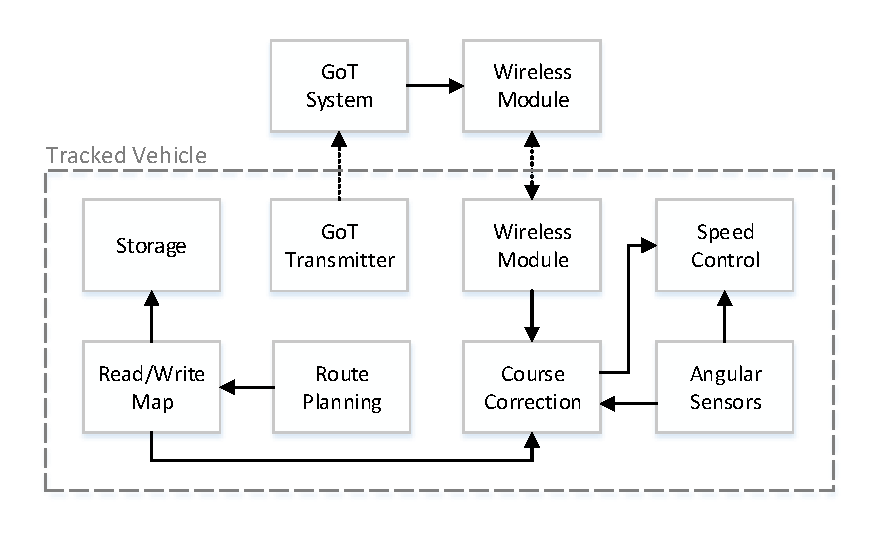
\includegraphics[scale=.9]{figures/systemOverview1}
%	\caption{Overview of the system prototype}
%	\label{fig:systemOverview1}
%\end{figure}

%The GoT system provides the vehicle with coordinates, which is utilized in course correction in combination with the map supplied from storage, to follow the route. In course correction lies also control between coordinates given by the GoT system and the storage, this is regulated through use of angular position and movement supplied by the angular sensors. The speed control gets an input from the course correction, the speed given is then held through regulation again using input from angular sensors, in this case specifically acceleration.


%Previously the rough prototype design is presented. To provide a more broad overview of the system, an exploded view of functionalities, their submodules and interfaces is presented in \figref{fig:systemOverview2}.

The overall functionalities for the project have been limited, due to time limitations and to focus on the scope of the project. A prototype will therefore be made to show the main functionalities necessary to make an automated vehicle containing principles for lawn mowing.\\
The final prototype includes a regulator, which will make it possible to follow a path from A to B. It is able to continue if the wireless connection is lost between the prototype and the GoT system for some duration. Furthermore it is able to plan a route within a given area and store these calculated data points locally, on the vehicle. The outline of the design is shown in \figref{fig:systemOverview2} to give an idea of the final prototype setup. In this section, the modules will be first presented, then the interfaces will describe the interaction between them.

\begin{figure}[H]
	\centering
	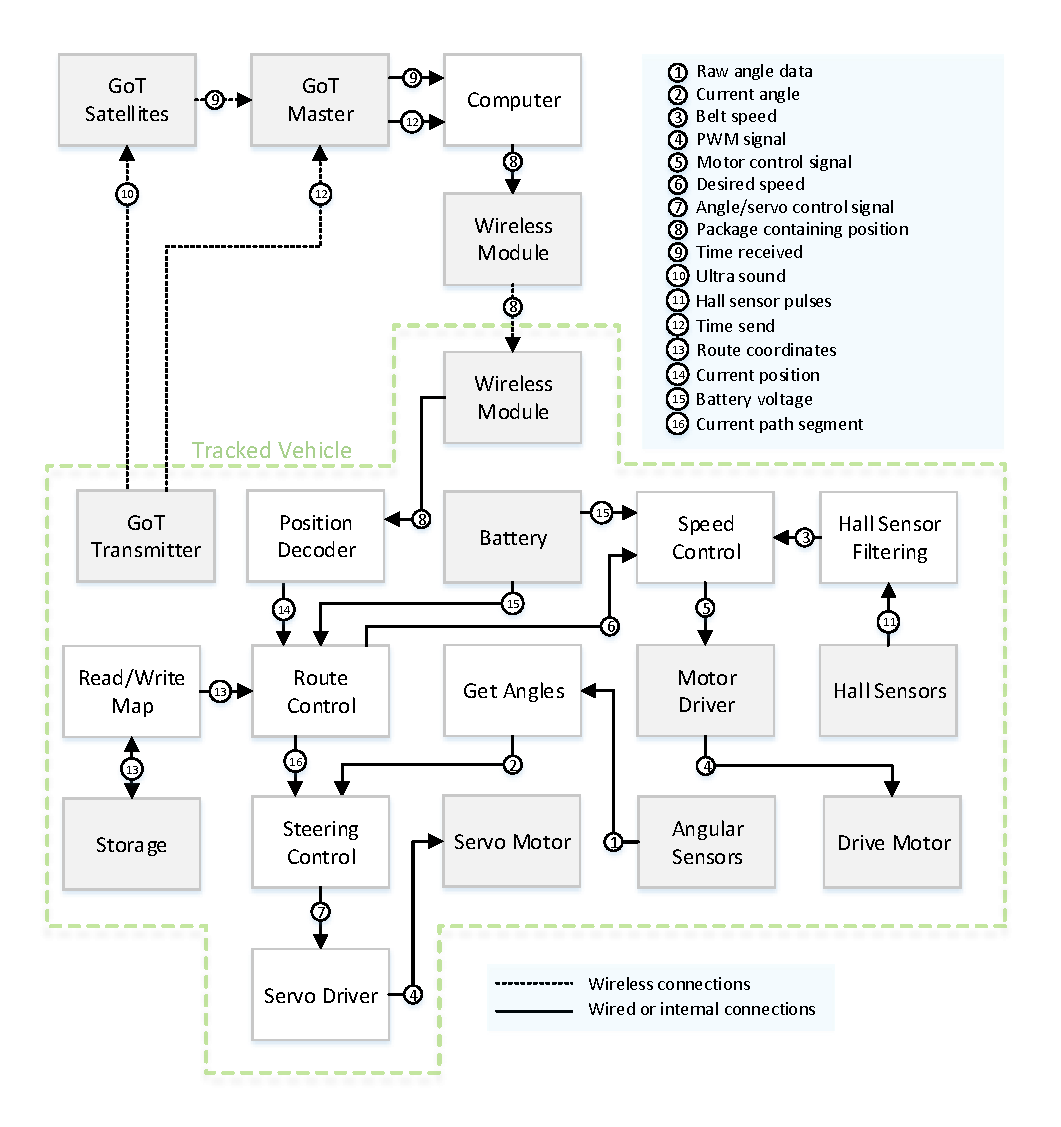
\includegraphics[scale=.9]{figures/systemOverview2}
	\caption{Overview of the softaware and electronic parts of the system prototype}
	\label{fig:systemOverview2}
\end{figure}
\todo{got transmitter instead of ultra sound and radio link, the 10 is also a time, the 12 and 9 are an electromagnetic signal}

\subsection{Modules}
In the following, apart from - \textit{Storage}, \textit{Read/Write Map} and \textit{Wireless Modules} - all the modules from the system prototype are described to understand the basis of the prototype.


\subsubsection{GoT System}
%The GoT satellites is placed in the area in which the vehicle needs to operate. These satellites receives information from the vehicle. The time which the vehicles transmitter sends out bursts is received by the GoT master. Furthermore the time which the satellites receives the information send from the vehicles transmitter is transmitted to the GoT master. The GoT master then relays the information received from the vehicle directly to the 

The \textit{GoT Transmitter} placed on the vehicle sends a signal containing the sended time to the \textit{GoT Satellites}, placed in the area in which the vehicle needs to operate, and to the \textit{GoT Master}. The satellites transmit the signal recieved to the master as soon as they recieve it. The master then relays those informations to the \textit{GoT on Computer} that will calculate the position of the car.


\subsubsection{Edge Map}
The first time the user will initialise the lawn mower, an \textit{Edge Map} will be created thanks to the GoT system. This edge map will determine the areas that the car is allowed to go or not, in regards of specifications or objects on the lawn.  

\subsubsection{Route Planning}
The Route Planning module calculates a route from the points gathered from the Edge Map. The route will be in straight lanes, as in the Bosch Logicut system \secref{roboMowers}, to guarantee that the whole lawn is cut. 

\subsubsection{Speed Control}
The speed is controled by the \textit{Hall Sensors} placed on the drive wheel. The submodule \textit{Get Speed} will relay this speed to the \textit{Speed Control} taking the belts into account. The new wanted speed will be sent to the \textit{Motor Driver}, which will finally instruct the \textit{Drive Motor} how to run.


\subsubsection{Angular Sensors}
The angular position is measured thanks to the \textit{Angular Sensors}, that will send data to the submodule \textit{Get Angle}, in charge to send the angle to the Speed Control and to the Course Correction submodule.

\subsubsection{Course Correction}
Thanks to all the informations from the different sensors for the speed, position, and angular position, the \textit{Course Correction} can decide how to react in consequence. It will send a instruction to the Speed Control and to the \textit{Servo Motor}, that will act directly on the steering of the vehicle, to try to stay on the desired path.

\subsection{Interfaces}
%- To Tom and Rasmus \newline
%In the subsection an explanation of the different interfaces between the modules is made. We have thought about making it like a high layer interface, where we only explain what we need the different modules to give each other. Like one module needs to get the map edge, i.e. coordinates, but since it is this early in the report and it would be more overview by writing map edge rather than coordinates. But as you can see in \figref{fig:systemOverview2} the layers of information are different, one is raw angle data and another time send. Is this okay or should we change something else?
%\indent
%The interfaces of the system is very important when designing each of the adjacent submodules. The existing interfaces as well as the ones presumed are also important in the process of analyzing the system capabilities width focus on requirements of the prototype. Width that in mind follows a brief review of the interfaces between each submodule.
In this section a high layer interface between the modules will be presented. This will help designing each of the adjacent submodules.

\subsubsection{GoT System Interfaces}
The GoT Transmitter sends the \textit{Time send} trough an \textit{Ultra sound} burst to the GoT Satellites, and trough an electromagnetic signal to the GoT Master. The same way, the GoT Satellites tranmits the \textit{Time received} by a electromagnetic signal to the GoT Master. The \textit{Position and time} will then be transmitted from the GoT Master to the GoT Computer, and then to the Wireless Module.

\subsubsection{Route Planning, Storage and Read/Write Map Interfaces}
The Edge Map submodule sends the \textit{Map edge} to Route Planning, that will send a \textit{Route} to Read/Write Map. The Route to follow will then be transmited to the Course Correction submodule for a path correction, and to the Storage for saving.

\subsubsection{Speed Control Interfaces}
The Hall Sensors send \textit{Hall sensor pulses} to the submodule Get Speed, that will process it to transmit the \textit{Belt speed} to the Speed Control. A \textit{PWM signal} containing the new wanted speed will then be sent to the Motor Driver, wich will convert it to the final \textit{Motor control signal} and sent it to the Drive Motor.

\subsubsection{Angular Sensors Interfaces}
The Angular Sensors will send a \textit{Raw angle data} to the submodule  Get Angles, that will process it and send the \textit{Processed angle data} to Course Correction.

\subsubsection{Course Correction Interfaces}
The Course Correction submodule receives the \textit{Position and Time} from the Wireless Module, the \textit{Route} to follow from Read/Write Map, and the \textit{Processed angle data} from Get Angles. With all those information, a decision will be sent to the Speed Control through the \textit{Desired speed}, and to the Servo Motor with an \textit{Angle/servo control signal}.\\\\


Now that the vehicle had been descibed and the prototype defined, the modelling of the vehicle can be made.


%---------------------------------------------------------------------------------------------------------------------------\\
%REWRITE THIS SCRAMBLED VERSION OF THE ABOVE TWO SUBSECTIONS \todo{rewrite in the above section and delete these subsections}\\
%---------------------------------------------------------------------------------------------------------------------------
%
%\subsubsection{GoT Satellites, Master and GoT Ultra Sound \& Radio Link}
%\indent
%A number of GoT Satellites are placed in the corners of the area in which the vehicle is to operate. These Satellites receive ultra sound signal from the GoT device placed on the vehicle. The time in which each ultrasound signal is received is passed through a wireless connection from the satellites to the GoT master. The GoT master then pairs this information with the time the ultra sound signal was send from the vehicle which it receives via radio link from the GoT device on the vehicle. After collecting the information, the GoT master sends a calculated position and along with a time stamp to the computer handling GoT.
%
%\subsubsection{Wireless Modules}
%\indent
%%The wireless modules serves the purpose of transmitting the calculated coordinates from the GoT system to the vehicle.
%
%\subsubsection{Edge Map, Route Planning, Read/Write Map and Storage}
%\indent
%%The route planning functionality receives the hard coded edge positions from edge map. Using this information the route is then planned and saved in the storage through the read/write map functionality.
%
%\subsubsection{Gyro, Accelerometer, Magnetometer, Speed Control and Course Correction}
%\indent
%%Gyro along with magnetometer is used for angular position of the vehicle. This is passed to the course correction through the get angle functionality. Here it is used as to correct the orientation of the vehicle on its path. The accelerometer also channels through the get angle functionality. The angular acceleration is then used for correction of the speed.
%
%\subsubsection{Hall Sensor}
%\indent
%%The speed control also receives input from the hall sensors through the get speed functionality, where the inputs from the hall sensors are translated to speed of the vehicle's belts. This information is then used in speed control to regulate the speed.
%
%\subsubsection{Servo Motor}
%\indent
%%The servo motor receives an angle/servo control signal from course correction. This angle equals a given amount of breaking on either of the two belts, which then through the differential gearing translate into steering and thus correction of the course of the vehicle.
%
%\subsubsection{Motor Driver and Drive Motor}
%\indent
%%The drive motor takes a motor control signal from the motor driver provided by the speed control. The control signal from speed control is a PWM signal.